
% JDR: This is probably more than 50 minutes worth of material.  A natural break
%   point is before the slides on Span.

\titleframe{Section 1.3}{Vector Equations}


%%%%%%%%%%%%%%%%%%%%%%%%%%%%%%%%%%%%%%%%%%%%%%%%%%%%%%%%%%%%%%%%%%%

\begin{frame}
\frametitle{Motivation}

We want to think about the \emph{algebra} in linear algebra (systems of
equations and their solution sets) in terms of \emph{geometry} (points, lines,
planes, etc).

\pause
\begin{center}
\def\r{\color{seq1}}\def\b{\color{seq2}}
$\syseq{\r x \r- \r3y \r= \r-3; \b2x \b+ \b y \b= \b8 }$
\qquad\longsquiggly\qquad
\begin{tikzpicture}[scale=.08, baseline]
  \draw[grid lines] (-20,-20) rectangle (20,20);
  \clip (-20,-20) rectangle (20,20);
  \draw[->] (-20,0) -- (20,0);
  \draw[->] (0,-20) -- (0,20);
  \draw[seq1, thick] (-20,-20/3+1) -- (20,20/3+1);
  \draw[seq2, thick] (-20,40+8) -- (20,-40+8);
  \point at (3,2);
\end{tikzpicture}
\end{center}

\bigskip
\pause
This will give us better insight into the properties of systems of equations and
their solution sets.

\bigskip
\pause
To do this, we need to introduce $n$-dimensional space $\R^n$, and
\textbf{vectors} inside it.

\end{frame}


%%%%%%%%%%%%%%%%%%%%%%%%%%%%%%%%%%%%%%%%%%%%%%%%%%%%%%%%%%%%%%%%%%%

\begin{frame}
\frametitle{Line, Plane, Space, $\ldots$}
Recall that $\R$ denotes the collection of all real numbers, i.e.\ the number
line.
\pause

\begin{defn}
  Let $n$ be a positive whole number.  We define
  \[ \R^n = \text{all ordered } n\text{-tuples of real numbers }
  (x_1,\,x_2,\,x_3,\,\ldots,\,x_n). \]
\end{defn}

\pause

\begin{eg}
  When $n=1$, we just get $\R$ back: $\R^1 = \R$.  Geometrically, this is the
  \emph{number line}.
  \begin{center}
    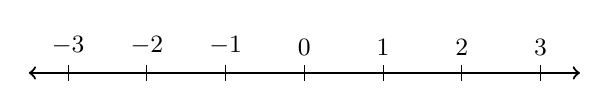
\begin{tikzpicture}
      \draw [<->, thick] (-3.5,0) -- (3.5,0);
      \foreach \x in {-3,...,3}
         \draw[thin] (\x,-.1) -- (\x,0.1) node[anchor=south] {\small$\x$};
    \end{tikzpicture}
  \end{center}
\end{eg}

\end{frame}


%%%%%%%%%%%%%%%%%%%%%%%%%%%%%%%%%%%%%%%%%%%%%%%%%%%%%%%%%%%%%%%%%%%

\begin{frame}
\frametitle{Line, Plane, Space, $\ldots$}
\framesubtitle{Continued}

\vskip-3mm
\begin{eg}
  When $n=2$, we can think of $\R^2$ as the \emph{plane}.  This is because every
  point on the plane can be represented by an ordered pair of real numbers,
  namely, its $x$- and $y$-coordinates.
  \vskip .5cm
  \begin{center}
    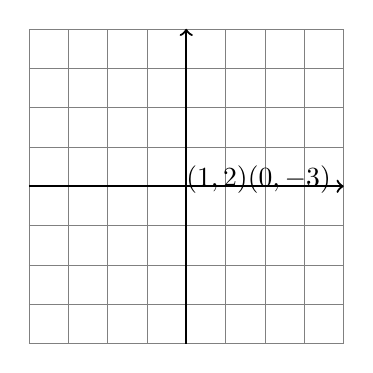
\begin{tikzpicture}[every node/.append style={whitebg, thin border},
        every label/.append style={text=seq-blue}, scale=.5]
      \draw[help lines] (-4, -4) grid (4, 4);
      \draw[->, thick] (-4,0) -- (4,0);
      \draw[->, thick] (0,-4) -- (0,4);
      \point[seq-blue, "{$(1,2)$}" above right] at (1,2);
      \point[seq-blue, "{$(0,-3)$}" above right] at (0,-3);
    \end{tikzpicture}
  \end{center}

  \pause We can use the elements of $\R^2$ to \emph{label} points on the
  plane, but $\R^2$ is not defined to be the plane!

\end{eg}

\end{frame}


%%%%%%%%%%%%%%%%%%%%%%%%%%%%%%%%%%%%%%%%%%%%%%%%%%%%%%%%%%%%%%%%%%%

\begin{frame}
\frametitle{Line, Plane, Space, $\ldots$}
\framesubtitle{Continued}

\vskip-3mm
\begin{eg}
  When $n=3$, we can think of $\R^3$ as the \emph{space} we (appear to) live
  in.  This is because every point in space can be represented by an ordered
  triple of real numbers, namely, its $x$-, $y$-, and $z$-coordinates.
  \vskip .5cm
  \begin{center}
    \begin{tikzpicture}[myxyz, scale=.5,
        every label/.append style={text=seq-blue}]
      \begin{scope}[transformxy]
        \draw[help lines] (-4, -4) grid (4, 4);
      \end{scope}
      \draw[->, thick] (-4,0,0) -- (4,0,0);
      \draw[->, thick] (0,-4,0) -- (0,4,0);
      \draw[->, thick] (0,0,0) -- (0,0,4);
      \draw[thick] (0,0,-4) -- (0,0,-2);
      \draw[thick,gray] (0,0,-2) -- (0,0,0);
      \draw[thin, densely dotted] (1,-1,3) -- (1,-1,0);
      \point[seq-blue, "${(1,-1,3)}$" above] at (1,-1,3);
      \draw[thin, densely dotted] (-2,2,2) -- (-2,2,0);
      \point[seq-blue, "${(-2,2,2)}$" above] at (-2,2,2);
    \end{tikzpicture}
  \end{center}

  \pause Again, we can use the elements of $\R^3$ to \emph{label} points in
  space, but $\R^3$ is not defined to be space!

\end{eg}

\end{frame}


%%%%%%%%%%%%%%%%%%%%%%%%%%%%%%%%%%%%%%%%%%%%%%%%%%%%%%%%%%%%%%%%%%%

\begin{frame}
\frametitle{Line, Plane, Space, $\ldots$}
\framesubtitle{Continued}

So what is $\R^4$?  or $\R^5$?  or $\R^n$?\\[2mm]
\pause\hskip 1em\ldots
go back to the \emph{definition}: ordered $n$-tuples of real numbers
\[ (x_1,x_2,x_3,\ldots,x_n). \]

\pause\bigskip
They're still ``geometric'' spaces, in the sense that our intuition for $\R^2$
and $\R^3$ sometimes extends to $\R^n$, but they're harder to visualize.

\pause\bigskip
We'll make definitions and state theorems that apply to any $\R^n$, but we'll
only draw pictures for $\R^2$ and $\R^3$.

\end{frame}


%%%%%%%%%%%%%%%%%%%%%%%%%%%%%%%%%%%%%%%%%%%%%%%%%%%%%%%%%%%%%%%%%%%

\begin{frame}
\frametitle{Vectors}
In the previous slides, we were thinking of elements of $\R^n$ as
\textbf{points}: in the line, plane, space, etc.

\pause\medskip
We can also think of them as \textbf{vectors}: arrows with a given length and
direction. 
\begin{center}
    \begin{tikzpicture}[scale=0.5, every pin/.style={whitebg, thin border}]
      \draw[grid lines] (-1,-1) grid (4, 4);
      \draw[->, thick] (-1,0) -- (4,0);
      \draw[->, thick] (0,-1) -- (0,4);
      \point[seq-blue, pin={
          [pin edge={seq-blue}, text=seq-blue, right]
          10:the point $(1,3)$}] (x) at (1,3);
      \draw[thick vector, green!50!black] (0,0)
        -- node[midway, pin={[right]-10:the vector $1\choose3$}] {} (x);
    \end{tikzpicture}
\end{center}
\pause
So the vector points \emph{horizontally} in the amount of its $x$-coordinate,
and \emph{vertically} in the amount of its $y$-coordinate.

\pause\medskip
When we think of an element of $\R^n$ as a vector, we write it as a matrix with
$n$ rows and one column:
\[ v = \vec{ 1 2 3}. \]
We'll see why this is useful later.

\note{Some authors use $\bb v$.}

\end{frame}


%%%%%%%%%%%%%%%%%%%%%%%%%%%%%%%%%%%%%%%%%%%%%%%%%%%%%%%%%%%%%%%%%%%

\begin{frame}
\frametitle{Points and Vectors}
So what is the difference between a point and a vector?%
\note{There isn't really any difference\ldots}

\pause\medskip
A vector need not start at the origin: \emph{it can be located anywhere\/}!
In other words, an arrow is determined by its length and its direction, not
by its location.\\[1mm]
\hbox to \linewidth{\hss
\begin{tikzpicture}[scale=0.5]
  \draw[help lines] (-1,-1) grid (4, 4);
  \draw[thick vector, seq-green] (0,1) -- (1,3);
  \draw[thick vector, seq-green] (1,1) -- (2,3);
  \draw[thick vector, seq-green] (2,0) -- (3,2);
  \node[anchor=west, text width=7.8cm] (a) at (5, 3.3)
    {These arrows all represent the vector $\color{seq-green}\vec{1 2}$.};
  \node<3->[below=.9cm of a.south west, anchor=west, bluebox, text width=7.5cm,
      inner sep=5pt, align=justify]
    {
      However, unless otherwise specified, we'll assume a vector starts
      at the origin: we'll usually be sloppy and identify the vector
      ${1\choose 2}$ with the point $(1,2)$.
    };
\end{tikzpicture}\hss}

\begin{uncoverenv}<4->\medskip
This makes sense in the real world: many physical quantities, such as velocity,
are represented as vectors.  But it makes more sense to think of the velocity of
a car as being located at the car.

\pause[5]\medskip
Another way to think about it: a vector is a \emph{difference} between two
points, or the arrow from one point to another.

\pause\medskip
For instance, $\vec{1 2}$ is the arrow from $(1,1)$ to $(2,3)$.\qquad
\begin{tikzpicture}[overlay, baseline=.75cm, scale=.5,
    whitebg nodes, thin border nodes]
  \draw[help lines] (0,0) grid (3,3);
  \draw[->] (0,0) -- (3,0);
  \draw[->] (0,0) -- (0,3);
  \point["${(1,1)}$" {left, text=seq-red}, seq-red] (x) at (1,1);
  \point["${(2,3)}$" {right, text=seq-green}, seq-green] (y) at (2,3);
  \draw[vector, seq-blue] (x)
    -- node[below right=1pt] {${1\choose 2}$} (y);
\end{tikzpicture}
\end{uncoverenv}

\end{frame}


%%%%%%%%%%%%%%%%%%%%%%%%%%%%%%%%%%%%%%%%%%%%%%%%%%%%%%%%%%%%%%%%%%%

\begin{frame}
\frametitle{Vector Algebra}

\vskip-3mm
\begin{defn}
  \begin{itemize}
  \item We can add two vectors together:
    \[ \vec{ a b c} + \vec{ x y z} = \vec{ a+x b+y c+z}. \]
    \pause
  \item We can multiply, or \textbf{scale}, a vector by a real number $c$:
    \[ \def\r{\textcolor{red}} \r c\vec{ x y z} 
    = \vec{ \r c\cdot x \r c\cdot y \r c\cdot z}. \]
    \pause
    We call $c$ a \textbf{scalar} to distinguish it from a vector.  If $v$ is a
    vector and $c$ is a scalar, $cv$ is called a \textbf{scalar multiple} of
    $v$.
  \end{itemize}
\end{defn}

\pause
(And likewise for vectors of length $n$.)
\pause
For instance,
\webonlycmd{
\[ \vec{ 1 2 3} + \vec{ 4 5 6} = \vec{ 5 7 9} \sptxt{and} 
-2\vec{ 1 2 3} = \vec{-2 -4 -6}. \]
}

\end{frame}


%%%%%%%%%%%%%%%%%%%%%%%%%%%%%%%%%%%%%%%%%%%%%%%%%%%%%%%%%%%%%%%%%%%

\begin{frame}
\frametitle{Vector Addition and Subtraction: Geometry}

\begin{center}
\vskip-4mm
\begin{tikzpicture}[scale=0.5]
  \draw[grid lines] (0,0) grid (5,5);
  \fill<5->[red!30, nearly transparent] (0,0) -- (1,3) -- (5,5) -- (4,2) -- cycle;
  \begin{scope}[thin border nodes]
  \draw<2->[vector, seq-blue] (0,0) to["$v$"] (1,3);
  \draw<3->[vector, seq-green] (1,3) to["$w$"] (5,5);
  \draw<2,5->[vector, seq-green] (0,0) to["$w$"'] (4,2);
  \draw<5->[vector, seq-blue] (4,2) to["$v$"'] (5,5);
  \draw<4->[vector] (0,0) to["$v+w$" {sloped, pos=.6}] (5,5);
  \end{scope}
  \draw<7->[|<->|] (0,5.5) -- (1,5.5);
  \draw<7->[|<->|] (1,5.5) -- (5,5.5);
  \draw<7->[|<->|] (0,-.5) -- (4,-.5);
  \draw<7->[|<->|] (4,-.5) -- (5,-.5);
  \path<7-> (0,-.5) -- (5,-.5)
     node[pos=.5, font=\small, below=1mm] {$5 = 1 + 4 = 4+1$};
  \draw<7->[|<->|] (5.5,0) -- (5.5,2);
  \draw<7->[|<->|] (5.5,2) -- (5.5,5);
  \draw<7->[|<->|] (-.5,0) -- (-.5,3);
  \draw<7->[|<->|] (-.5,3) -- (-.5,5);
  \path<7-> (-.5, 0) -- (-.5, 5)
     node[pos=.5, font=\small, above, rotate=90] {$5 = 2 + 3 = 3 + 2$};
  \node[anchor=north west] at (6.5,6) {
     \begin{minipage}{0.6\linewidth}
       \def\v{\textcolor{seq-blue}v}\def\w{\textcolor{seq-green}w}
       \alert{\large The parallelogram law for vector addition}\\[1mm]%
       \pause
       Geometrically, the sum of two vectors 
       $\v,\w$ is obtained as follows:
       \pause
       place the tail of $\w$ at the head of $\v$.  
       \pause
       Then $v+w$ is the vector whose tail is the tail of $\v$ and whose head is
       the head of $\w$.
       \pause
       Doing this both ways creates a \textcolor{red!60}{parallelogram}.
       \pause
       For example,
       \[ \textcolor{seq-blue}{\vec{1 3}}
       + \textcolor{seq-green}{\vec{4 2}}
       = \vec{5 5}. \]
       \pause
       Why?  The width of $v+w$ is the sum of the widths, and likewise with
       the heights.
     \end{minipage}
   };
  \useasboundingbox (-1.5,-1.5) rectangle (6,6);
\end{tikzpicture}
\end{center}
\note{Mention commutativity}

\begin{uncoverenv}<8->
\begin{center}
\vskip-2mm
\begin{tikzpicture}[scale=0.5]
  \draw[grid lines] (0,0) grid (5,5);
  \begin{scope}[thin border nodes]
  \draw<9->[vector, seq-blue] (0,0) to["$v$"] (1,4);
  \draw<9->[vector, seq-green] (0,0) to["$w$"] (4,2);
  \draw<11->[vector] (4,2) to["$v-w$"' {sloped, pos=.7}] (1,4);
  \end{scope}
  \node[anchor=north west] at (6.5,6) {
     \begin{minipage}{0.6\linewidth}
       \def\v{\textcolor{seq-blue}v}\def\w{\textcolor{seq-green}w}
       \alert{\large Vector subtraction}\\[1mm]%
       \pause[9]%
       Geometrically, the difference of two vectors 
       $\v,\w$ is obtained as follows:
       \pause
       place the tail of $\v$ and $\w$ at the
       same point.
       \pause
       Then $v-w$ is the vector from the head of $\v$ to the head of $\w$. 
       \pause
       For example,
       \[ \textcolor{seq-blue}{\vec{1 4}}
       - \textcolor{seq-green}{\vec{4 2}}
       = \vec{-3 2}. \]
       \pause
       Why?  If you add $v-w$ to $\w$, you get $\v$.
     \end{minipage}
   };
  \useasboundingbox (-1.5,-1.5) rectangle (6,6);
\end{tikzpicture}\qquad
\end{center}
\end{uncoverenv}

\begin{uncoverenv}<14->
  \vskip-5mm
  This works in higher dimensions too!\qquad
  \begin{tikzpicture}[scale=.25, myxyz, overlay, baseline=4mm]
    \begin{scope}[transformxy]
      \draw[grid lines] (-1, -4) grid (4, 1);
    \end{scope}
    \fill[red!30, nearly transparent] (0,0,0) -- (2,-1,.5) --
      (3,-2,3.5) -- (1,-1,3) -- cycle;
    \draw[vector,seq-blue] (0,0,0) -- (1,-1,3);
    \draw[thin,densely dotted] (1,-1,3) -- (1,-1,0);
    \draw[vector,seq-green] (1,-1,3) -- (3,-2,3.5);
    \draw[thin,densely dotted] (3,-2,3.5) -- (3,-2,0);
    \draw[vector,seq-green] (0,0,0) -- (2,-1,.5);
    \draw[thin,densely dotted] (2,-1,.5) -- (2,-1,0);
    \draw[vector,seq-blue] (2,-1,.5) -- (3,-2,3.5);
    \draw[vector] (0,0,0) -- (3,-2,3.5);
  \end{tikzpicture}
  
\end{uncoverenv}

\end{frame}


%%%%%%%%%%%%%%%%%%%%%%%%%%%%%%%%%%%%%%%%%%%%%%%%%%%%%%%%%%%%%%%%%%%

\begin{frame}
\frametitle{Scalar Multiplication: Geometry}
\alert{Scalar multiples of a vector}\\
These have the same \emph{direction} but a different \emph{length}.

\note{Ask where $2v$, $-\frac 12v$, $0v$ are.}

\begin{center}
  \begin{tikzpicture}[scale=0.5, baseline=.8cm]
    \draw[grid lines] (-2,-2) grid (3,5);
    \node[anchor=south] at (.5,5) {Some multiples of $v$.};
    \draw[vector] (0,0) -- (1,2) node[below right, whitebg] {$v$};
    \begin{webonly}
    \draw[vector] (0,0) -- (2,4) node[below right, whitebg] {$2v$};
    \draw[vector] (0,0) -- (-.5,-1) node[left, whitebg] {$-\frac 12v$};
    \point["$0v$" below right] at (0,0);
    \end{webonly}
  \end{tikzpicture}
  \quad
  $\displaystyle\begin{aligned}[c]
    v &= \vec{1 2} \\
    2v &= \vec{2 4} \\
    -\frac 12v &= \vec{-\frac 12, -1} \\
    0v &= \vec{0 0}
  \end{aligned}$
  \quad\;\pause
  \begin{tikzpicture}[scale=0.5, baseline=.8cm]
    \node[anchor=south] at (.5,5) {All multiples of $v$.};
    \draw[help lines] (-2,-2) grid (3,5);
    \pause
    \draw[thick, seq-blue, <->] (-1,-2) -- (2.5, 5);
    \point at (0,0);
  \end{tikzpicture}
\end{center}

\bigskip
\uncover<4->
{So the scalar multiples of $v$ form a \emph{line}.}

\end{frame}


%%%%%%%%%%%%%%%%%%%%%%%%%%%%%%%%%%%%%%%%%%%%%%%%%%%%%%%%%%%%%%%%%%%

\begin{frame}
\frametitle{Linear Combinations}
We can add and scalar multiply in the same equation:
\pause
\[ w = c_1v_1 + c_2v_2 + \cdots + c_pv_p \]
where $c_1,c_2,\ldots,c_p$ are \blankuntil{3}{scalars},
\pause
$v_1,v_2,\ldots,v_p$ are \blankuntil{4}{vectors}
\pause
in $\R^n$, and $w$ is a
\blankuntil{5}{vector}
\pause
in $\R^n$.

\pause
\begin{defn}
  We call $w$ a \textbf{linear combination} of the vectors
  $v_1,v_2,\ldots,v_p$. 
  \pause
  The scalars $c_1,c_2,\ldots,c_p$ are called the
  \textbf{weights} or \textbf{coefficients}.
\end{defn}

\pause
\begin{eg}
  \begin{tikzpicture}[scale=0.5, thin border nodes]
    \draw[help lines] (-3,-3) grid (4, 4);
    \draw[->] (-3,0) -- (4,0);
    \draw[->] (0,-3) -- (0,4);
    \draw[vector, seq1] (0,0) to["$v$"] (1,2);
    \draw[vector, seq2] (0,0) to["\strut$w$"'] (1,0);
    \point at (0,0);
    \begin{webonly}
    \point[seq3] at (2,2);
    \point[seq4] at (0,2);
    \point[seq5] at (2,4);
    \point[seq8] at (2,0);
    \point[seq7] at (-1,-2);
    \end{webonly}

    \node[anchor=west] at (5, .75)
      {
        \begin{minipage}{0.6\linewidth}
           Let $\color{seq1}v = \vec{ 1 2}$ and 
           $\color{seq2}w = \vec{ 1 0}$.\\[1mm]
           What are some linear combinations
           of $v$ and $w?$
           \begin{itemize}
           \item $\color{seq3} v+w$
           \item $\color{seq4} v-w$
           \item $\color{seq5} 2v\color{gray}+0w$
           \item $\color{seq8} 2w$
           \item $\color{seq7} -v$
           \end{itemize}
        \end{minipage}
      };
    
  \end{tikzpicture}
\end{eg}

\end{frame}


%%%%%%%%%%%%%%%%%%%%%%%%%%%%%%%%%%%%%%%%%%%%%%%%%%%%%%%%%%%%%%%%%%%

\begin{pollframe}

\begin{bluebox}[Poll]{.6\textwidth}
  Is there any vector in $\R^2$ that is \emph{not} a linear combination of $v$
  and $w$?
\end{bluebox}

\medskip
\begin{uncoverenv}<2->
  No: in fact, \emph{every} vector in $\R^2$ is a combination of $v$ and $w$.
\end{uncoverenv}


\begin{center}
  \begin{tikzpicture}[scale=0.5]
    \draw<1>[grid lines] (-3,-3) grid (3,3);
    \path<2->[clip] (-3,-3) rectangle (3, 3);
    \filldraw<2->[grid lines, fill=seq4!30!white] (-3,-3) rectangle (3, 3);
    \begin{scope}
      \pgftransformcm {1}{0}{1}{2}{\pgfpoint{0cm}{0cm}}
      \draw<2->[very thin, seq4] (-6,-2) grid (6,2);
    \end{scope}
    \draw[vector, seq1] (0,0) --
      node [midway, above left=-2pt] {$v$} (1,2);
    \draw[vector, seq2] (0,0) --
      node [midway, below] {$w$} (1,0);
    \point at (0,0);
  \end{tikzpicture}
\end{center}

\uncover<3->{
  (The purple lines are to help measure \emph{how much} of $v$ and $w$ you need to
  get to a given point.)
}

\end{pollframe}


%%%%%%%%%%%%%%%%%%%%%%%%%%%%%%%%%%%%%%%%%%%%%%%%%%%%%%%%%%%%%%%%%%%

\begin{frame}
\frametitle{More Examples}

\begin{tikzpicture}[scale=0.5]
  \begin{scope}
    \draw[grid lines] (-3,-3) grid (4, 4);
    \clip (-3,-3) rectangle (4, 4);
    \begin{webonly}
    \draw[thin, seq4] ($-2*(2,1)$) -- ($2*(2,1)$);
    \point[seq2] at (3,1.5);
    \point[seq3] at (-1, -.5);
    \end{webonly}
    \draw[vector, seq1] (0,0) to["$v$" thin border] (2,1);
    \point at (0,0);
  \end{scope}

  \node[anchor=west] at (5, .75)
    {
      \begin{minipage}{0.6\linewidth}
        What are some linear combinations of $\color{seq1}v = \vec{2 1}$?
        \begin{webonly}
        \begin{itemize}
        \item $\color{seq2} \frac 32v$
        \item $\color{seq3} -\frac 12v$
        \item $\ldots$
        \end{itemize}

        \smallskip
        What are \emph{all} linear combinations of $v$?\\[1mm]%
        All vectors $cv$ for $c$ a real number.
        I.e., all \emph{scalar multiples} of $v$.
        These form a \emph{line}.
        \end{webonly}
      \end{minipage}
    };
\end{tikzpicture}

\medskip

\begin{uncoverenv}<2->
\begin{tikzpicture}[scale=0.5]
  \begin{scope}
    \draw[grid lines] (-3,-3) grid (4, 4);
    \path[clip] (-3,-3) rectangle (4, 4);
    \draw<3->[thin, seq4] ($-2*(2,2)$) -- ($2*(2,2)$);
    \draw[vector, seq1] (0,0) to["$v$" thin border] (2,2);
    \draw[vector, seq2] (0,0) to["$w$"' thin border] (-1,-1);
    \point at (0,0);
  \end{scope}

  \node[anchor=west] at (5, .75)
    {
      \begin{minipage}{0.6\linewidth}
        \begin{ques}
          What are all linear combinations of 
          \[ \textcolor{seq1}{v = \vec{2 2}} \sptxt{and}
          \textcolor{seq2}{w = \vec{-1 -1}}? \]
        \end{ques}
        \uncover<3->{\alert{Answer:} The line which contains both vectors.}
        
        \medskip
        \uncover<4->{What's different about this example and the one on the poll?}
      \end{minipage}
    };
\end{tikzpicture}
\end{uncoverenv}

\end{frame}


%%%%%%%%%%%%%%%%%%%%%%%%%%%%%%%%%%%%%%%%%%%%%%%%%%%%%%%%%%%%%%%%%%%

\begin{frame}
\frametitle{Systems of Linear Equations}

\vskip-3mm
\begin{ques}
  Is $\vec{ 8 16 3}$ a linear combination of $\vec{1 2 6}$ and $\vec{-1 -2 -1}$?
\end{ques}

\smallskip
\begin{webonly}%
\alert{This means:} can we solve the equation
\[ x\vec{1 2 6} + y \vec{-1 -2 -1} = \vec{8 16 3} \]
where $x$ and $y$ are the unknowns (the coefficients)?
Rewrite:
\[ \vec{ x 2x 6x} + \vec{-y -2y -y} = \vec{8 16 3}
\qquad\text{or}\qquad
\spalignsysdelims()\syseq{ x - y; 2x - 2y; 6x - y} = \vec{8 16 3}. \]
This is just a system of linear equations:
\[ \syseq{x - y = 8; 2x - 2y = 16; 6x - y = 3\rlap.} \]
\end{webonly}

\end{frame}


%%%%%%%%%%%%%%%%%%%%%%%%%%%%%%%%%%%%%%%%%%%%%%%%%%%%%%%%%%%%%%%%%%%

\begin{frame}
\frametitle{Systems of Linear Equations}

\def\r{\color<7->{seq-red}}
\def\g{\color<7->{seq-green}}
\def\b{\color<7->{seq-blue}}

\framesubtitle{Continued}
\hfill$\syseq{x - y = 8; 2x - 2y = 16; 6x - y = 3}$\qquad\pause
\hbox to .6\hsize{\longsquiggly[matrix form] \hfill
  $\amat{\r1 \g-1 \b8; \r2 \g-2 \b16; \r6 \g-1 \b3}$\hskip 1cm}\\[1mm]%
\pause\hfill
\hbox to .6\hsize{\longsquiggly[row reduce]\hfill
  $\amat{1 0 -1; 0 1 -9; 0 0 0}$\hskip 1cm}\\[1mm]%
\pause\hfill
\hbox to .6\hsize{\longsquiggly[solution]\hfill
  $\syseq{x = -1; y = -9}$ \hskip 1.3cm}

\pause
Conclusion:
\[ -{\r\vec{1 2 6}} - 9{\g\vec{-1 -2 -1}} = {\b\vec{8 16 3}} \]

\pause\medskip
What is the relationship between the original vectors and the matrix form of the
linear equation? \pause They have the same columns!

\pause\bigskip
\alert{Shortcut:} You can make the augmented matrix without writing down the
system of linear equations first.

\end{frame}


%%%%%%%%%%%%%%%%%%%%%%%%%%%%%%%%%%%%%%%%%%%%%%%%%%%%%%%%%%%%%%%%%%%

\begin{frame}
\frametitle{Vector Equations and Linear Equations}

\vskip-7mm\null
\begin{bluebox}[Summary]{.8\textwidth}
  The vector equation
  \[ x_1v_1 + x_2v_2 + \cdots + x_p v_p = b, \]
  where $v_1,v_2,\ldots,v_p,b$ are vectors in $\R^n$ and $x_1,x_2,\ldots,x_p$
  are scalars, \uncover<2->{%
  has the same solution set as the linear system with augmented matrix
  \[ \amat[c]{| | ,, | |; v_1 v_2 \cdots, v_p b; | | ,, | |}, \]
  where the $v_i$'s and $b$ are the columns of the matrix.}
\end{bluebox}

\pause[3]%
So we now have (at least) \emph{two} equivalent ways of thinking about linear
systems of equations:
\begin{enumerate}
  \pause
\item Augmented matrices.
  \pause
\item Linear combinations of vectors (vector equations).
\end{enumerate}

\pause
The last one is more geometric in nature.

\note{In math, you always want several different but equivalent ways of thinking
  about the same problem---because that gives you more ways to solve it!}

\end{frame}


%%%%%%%%%%%%%%%%%%%%%%%%%%%%%%%%%%%%%%%%%%%%%%%%%%%%%%%%%%%%%%%%%%%

\begin{frame}
\frametitle{Span}

It is important to know what are \emph{all\/} linear combinations of a set of
vectors $v_1,v_2,\ldots,v_p$ in $\R^n$: \pause it's exactly the collection of all $b$
in $\R^n$ such that the vector equation (in the unknowns $x_1,x_2,\ldots,x_p$)
\displayskips{3pt}
\[ x_1v_1 + x_2v_2 + \cdots + x_pv_p = b \]
has a solution (i.e., is consistent).

\pause
\medskip

\begin{defn}
  Let $v_1,v_2,\ldots,v_p$ be vectors in $\R^n$.  The \textbf{span} of
  $v_1,v_2,\ldots,v_p$ is the collection of all linear combinations of
  $v_1,v_2,\ldots,v_p$, and is denoted $\Span\{v_1,v_2,\ldots,v_p\}$. \pause
  In symbols:
  \begin{center}
    \namedbox{redbox}{
        $\displaystyle\Span\{v_1,v_2,\ldots,v_p\} =
        \namedbox{begin set}{\bigl\{{}} \,x_1v_1+x_2v_2+\cdots+x_pv_p
        \namedbox{such that}{{}\bigm|{}} x_1,x_2,\ldots,x_p\text{ in }\R \,\bigr\}$.
        }
  \end{center}
  \note{Translate the symbols back to words.}
  \uncover<6->{
  \alert{Synonyms:} $\Span\{v_1,v_2,\ldots,v_p\}$ is the subset \textbf{spanned by} or
  \textbf{generated by} $v_1,v_2,\ldots,v_p$.
  }
\end{defn}

\smallskip
\begin{uncoverenv}<5->
\begin{tikzpicture}[remember picture]
  \node<7->[overlay, redbox, fit=(redbox), inner sep=5pt] (x) {};
  \node<7->[bluebox, text width=.9\textwidth, font=\normalsize, align=justify]
    (bluebox) at (0,0)
  {
    This is the first of several definitions in this class that you simply
    \textbf{must learn}.  I will give you other ways to think about Span, and ways
    to draw pictures, but \emph{this is the definition}.  Having a vague idea what
    Span means will not help you solve any exam problems!
  };
  \begin{scope}[overlay]
  \draw<7->[->, very thick, shorten >=1pt, rounded corners] 
    (bluebox.west)
      -- ($(bluebox.west -| current page.west)!.3cm!(bluebox.west)$)
      |- (x.west);
  \node<5->[above=1.6cm of such that.north, xshift=.3cm, blue!50] (stlabel)
    {``such that''};
  \draw<5->[->, shorten >=1pt, blue!50]
    (stlabel) to[in=90,out=-90] (such that.north);
  \node<5->[above=1.6cm of begin set.north, xshift=-.3cm, blue!50] (setlabel)
    {``the set of''};
  \draw<5->[->, shorten >=1pt, blue!50]
    (setlabel) to[in=90,out=-90] (begin set.north);
  \end{scope}
  
\end{tikzpicture}
\end{uncoverenv}
\vss

\end{frame}


%%%%%%%%%%%%%%%%%%%%%%%%%%%%%%%%%%%%%%%%%%%%%%%%%%%%%%%%%%%%%%%%%%%

\begin{frame}
\frametitle{Span}
\framesubtitle{Continued}

Now we have several equivalent ways of making the same statement:
\begin{enumerate}
\pause
\item A vector $b$ is in the span of $v_1,v_2,\ldots,v_p$.
\pause
\item The linear system with augmented matrix
  \[ \amat[c]{| | ,, | |; v_1 v_2 \cdots, v_p b; | | ,, | |} \]
  is consistent.
\pause
\item The vector equation
  \[ x_1v_1 + x_2v_2 + \cdots + x_pv_p = b \]
  has a solution.
\end{enumerate}

\pause\bigskip
\alert{Note:} \textbf{equivalent} means that, for any given list of vectors
$v_1,v_2,\ldots,v_p,b$, \emph{either} all three statements are true,
\emph{or} all three statements are false.

\end{frame}


%%%%%%%%%%%%%%%%%%%%%%%%%%%%%%%%%%%%%%%%%%%%%%%%%%%%%%%%%%%%%%%%%%%

\begin{frame}
\frametitle{Pictures of Span}

Drawing a picture of $\Span\{v_1,v_2,\ldots,v_p\}$ is the same as drawing a picture
of all linear combinations of $v_1,v_2,\ldots,v_p$.

\pause
\bigskip
\hfill
\begin{tikzpicture}[scale=0.5, thin border nodes]
  \draw[grid lines] (-3,-2) grid (4, 3);
  \path[clip] (-3,-2) rectangle (4, 3);
  \draw<3->[thin, seq4] ($-2*(2,1)$) -- ($2*(2,1)$);
  \node<3->[seq4,whitebg] at (0,2) {$\Span\{v\}$};
  \draw[vector, seq1] (0,0) to["$v$"] (2,1);
  \point at (0,0);
\end{tikzpicture}
\hfill
\pause[4]%
\begin{tikzpicture}[scale=0.5, thin border nodes]
  \draw[grid lines] (-3,-2) grid (4, 3);
  \fill<5->[seq4!30, nearly transparent] (-3,-2) rectangle (4,3);
  \node<5->[seq4] at (.5,2.5) {$\Span\{v,w\}$};
  \draw[vector, seq1] (0,-1) to["$v$"] (1,1);
  \draw[vector, seq2] (0,-1) to["\strut$w$"'] (1,-1);
  \point at (0,-1);
\end{tikzpicture}
\hfill\null

\bigskip
\pause[6]%
\hfill
\begin{tikzpicture}[scale=0.5, thin border nodes]
  \draw[grid lines] (-3,-3) grid (4, 4);
  \path[clip] (-3,-3) rectangle (4, 4);
  \node<7->[seq4] at (.5,2.5) {$\Span\{v,w\}$};
  \draw<7->[thin, seq4] ($-2*(2,2)$) -- ($2*(2,2)$);
  \draw[vector, seq1] (0,0) to["$v$"] (2,2);
  \draw[vector, seq2] (0,0) to["$w$"' pos=.4] (-1,-1);
  \point at (0,0);
\end{tikzpicture}
\hfill\null

\end{frame}


%%%%%%%%%%%%%%%%%%%%%%%%%%%%%%%%%%%%%%%%%%%%%%%%%%%%%%%%%%%%%%%%%%%

\begin{frame}
\frametitle{Pictures of Span}
\framesubtitle{In $\R^3$}

\hfill
\begin{tikzpicture}[myxyz, scale=0.5, thin border nodes]
  \path[clip, resetxy] (-4,-3) rectangle (4,3);

  \draw<2->[seq4] ($-3*(2,-1,1)$) -- (0,0,0);

  \begin{scope}[transformxy]
    \fill[white, nearly opaque] (-2, -2) rectangle (3, 3);
    \draw[grid lines] (-2, -2) grid (3, 3);
  \end{scope}

  \draw<2->[seq4] (0,0,0) -- ($3*(2,-1,1)$);
  \node<2->[seq4] at (-1cm, 2cm) {$\Span\{v\}$};

  \draw[vector, seq1] (0,0,0) to["$v$"] (2,-1,1);
  \draw[thin, densely dotted] (2,-1,1) -- (2,-1,0);

  \point at (0,0,0);

\end{tikzpicture}
\hfill
\begin{uncoverenv}<3->
\begin{tikzpicture}[myxyz, scale=0.5, thin border nodes]
  \path[clip, resetxy] (-4,-3) rectangle (4,3);

  \def\v{(2,-1,1)}
  \def\w{(2,1,.3)}

  \node[coordinate] (X) at \v {};
  \node[coordinate] (Y) at \w {};

  \begin{scope}[x=(X), y=(Y), transformxy]
    \path[clip] (-1.5, 5) -- (1.5, -5) -- (1.5, -7) -- (-1.5, -7) -- cycle;
    \fill<4->[seq4!30, nearly opaque] (-1.5,-1) rectangle (1.5,2);
    \draw<4->[step=.5cm, seq4, very thin] (-1.5,-1) grid (1.5,2);
  \end{scope}

  \begin{scope}[transformxy]
    \fill[white, nearly opaque] (-2, -2) rectangle (3, 3);
    \draw[grid lines] (-2, -2) grid (3, 3);
  \end{scope}

  \begin{scope}[x=(X), y=(Y), transformxy]
    \path[clip] (-1.5, 5) -- (1.5, -5) -- (1.5, 7) -- (-1.5, 7) -- cycle;
    \fill<4->[seq4!30, nearly opaque] (-1.5,-1) rectangle (1.5,2);
    \draw<4->[step=.5cm, seq4, very thin] (-1.5,-1) grid (1.5,2);
  \end{scope}

  \node<4->[seq4] at (-1cm, 2cm) {$\Span\{v,w\}$};

  \draw[vector, seq1] (0,0,0) -- 
    node [midway, above] {$v$} \v;
  \draw[thin, densely dotted] \v -- \projxy\v;
  \draw[vector, seq2] (0,0,0) -- 
    node [midway, below] {\strut$w$} \w;
  \draw[thin, densely dotted] \w -- \projxy\w;

  \point at (0,0,0);

\end{tikzpicture}
\end{uncoverenv}
\hfill\null

\medskip
\hfill
\begin{uncoverenv}<5->
\begin{tikzpicture}[myxyz, scale=0.5, thin border nodes]
  \path[clip, resetxy] (-4,-3) rectangle (4,3);

  \begin{scope}[transformxy]
    \fill[white, nearly opaque] (-2, -2) rectangle (3, 3);
    \draw[grid lines] (-2, -2) grid (3, 3);
  \end{scope}

  \draw[vector, seq1] (0,0,0) to["$v$"] (2,-1,1);
  \draw[thin, densely dotted] (2,-1,1) -- (2,-1,0);
  \draw[vector, seq2] (0,0,0) to["\strut$w$"'] (2,1,.3);
  \draw[thin, densely dotted] (2,1,.3) -- (2,1,0);
  \draw[vector, seq3] (0,0,0) to["$u$"] (-.5,.5,1);
  \draw[thin, densely dotted] (-.5,.5,1) -- (-.5,.5,0);

  \point at (0,0,0);

  \fill<6->[seq4!30, nearly transparent, resetxy] (-4,-3) rectangle (4,3);
  \node<6->[seq4] at (-1cm, 2cm) {$\Span\{u,v,w\}$};

\end{tikzpicture}
\end{uncoverenv}
\hfill
\begin{uncoverenv}<7->
\begin{tikzpicture}[myxyz, scale=0.5, thin border nodes]
  \path[clip, resetxy] (-4,-3) rectangle (4,3);

  \def\v{(2,-1,1)}
  \def\w{(2,1,.3)}
  \def\u{(2,0,.65)}

  \node[coordinate] (X) at \v {};
  \node[coordinate] (Y) at \w {};

  \begin{scope}[x=(X), y=(Y), transformxy]
    \path[clip] (-1.5, 5) -- (1.5, -5) -- (1.5, -7) -- (-1.5, -7) -- cycle;
    \fill<8->[seq4!30, nearly opaque] (-1.5,-1) rectangle (1.5,2);
    \draw<8->[step=.5cm, seq4, very thin] (-1.5,-1) grid (1.5,2);
  \end{scope}

  \begin{scope}[transformxy]
    \fill[white, nearly opaque] (-2, -2) rectangle (3, 3);
    \draw[grid lines] (-2, -2) grid (3, 3);
  \end{scope}

  \begin{scope}[x=(X), y=(Y), transformxy]
    \path[clip] (-1.5, 5) -- (1.5, -5) -- (1.5, 7) -- (-1.5, 7) -- cycle;
    \fill<8->[seq4!30, nearly opaque] (-1.5,-1) rectangle (1.5,2);
    \draw<8->[step=.5cm, seq4, very thin] (-1.5,-1) grid (1.5,2);
  \end{scope}

  \node<8->[seq4] at (-1cm, 2cm) {$\Span\{u,v,w\}$};

  \draw[vector, seq1] (0,0,0) -- 
    node [midway, above] {$v$} \v;
  \draw[thin, densely dotted] \v -- \projxy\v;
  \draw[vector, seq2] (0,0,0) -- 
    node [midway, below] {\strut$w$} \w;
  \draw[thin, densely dotted] \w -- \projxy\w;
  \draw[vector, seq3] (0,0,0) -- 
    \u node [right] {$u$};
  \draw[thin, densely dotted] \u -- \projxy\u;

  \draw[thin, densely dotted] \v -- \w;

  \point at (0,0,0);

\end{tikzpicture}
\end{uncoverenv}
\hfill\null

\end{frame}


%%%%%%%%%%%%%%%%%%%%%%%%%%%%%%%%%%%%%%%%%%%%%%%%%%%%%%%%%%%%%%%%%%%

\begin{pollframe}

\medskip
\begin{bluebox}[Poll]{.6\textwidth}
  How many vectors are in $\Span\left\{ \vec{0 0 0} \right\}$?  
  \begin{enumerate}
    \renewcommand{\theenumi}{\Alph{enumi}}
  \item Zero
  \item One
  \item Infinity
  \end{enumerate}
\end{bluebox}

\pause\bigskip
In general, it appears that $\Span\{v_1,v_2,\ldots,v_p\}$ is the smallest ``linear
space'' (line, plane, etc.) containing the origin and all of the vectors
$v_1,v_2,\ldots,v_p$.

\pause\bigskip
We will make this precise later.

\note{Ask: what is the definition of Span?}

\end{pollframe}


%%% Local Variables:
%%% TeX-master: "../slides"
%%% End:
